%!TEX root = main.tex
\chapter{Implementation}
\label{chap:impl}

\section{The Algorithm}

Several depth estimation algorithms have been described in section
\ref{sec:depthestimation_theory}. A block matching algorithm
\texttt{[TODO: reference to some paper. Other than the taxonomy, for
  some variation!]} was chosen due to it's simplicity, decent quality
and speed. Since it is a local algorithm \texttt{[TODO: reference the
  taxonomy paper]}, it is very data parallel and well suited for the
GPU architecture.

The algorithm can be viewed as a pipeline containing the rough steps:

\begin{enumerate}
\item Correlation cost
\item Aggregation of costs
\item Disparity selection
\item Refinement and post-processing
\end{enumerate}

This chapter will present basic and optimized versions of each of
these steps, and a short conclusion for why a version was chosen for
the final real time algorithm.

\section{Overview}

The block matching algorithm has an O(1) complexity. But for HD input,
the amount of calculations is still large enough for it to not run in
real time, unless heavy optimizations are applied.

A simple version of a block matching algorithm would have to calculate
the pipeline for $H \times W \times D$ pixels. For an algorithm with
an $N \times N$ aggregation window, the number of calculations for a
pipeline would be $N \times N \times 3$. In total, $H \times W \times
D \times N \times N \times 3$. For a $1024 \times 768$ image, $9
\times 9$ aggregation window and $255$ disparity search range,
calculations are needed. For stereo depth maps, twice that is needed.
And for real tdsime (25 fps) videos, multiply that with 40.


\subsection{Assumptions}

The input images need to be stereo rectified single channel 8-bit
grayscale.

For the diffing to be effective, the camera rig and scene should be
stationary. Less foreground objects moving on the scene will result in
faster run times.

No non-Lambertian surfaces. That is, the surface needs to reflect the
same apparent brightness from all perspectives. Will result in
matching errors.

Note: All code listings are simplified. Boundry checks, variable
declarations and function signatures are mostly excluded.
\texttt{[TODO: Should the code listings be simplified?]}

\section{CPU Implementation}

The CPU implementation is a proof-of-concept, rather than a usable
prototype, to set the bar for a serious GPU implementation. It is
possible to heavily optimize it, but it will most likely never reach
real time on current commodity hardware. It was made to clearly
outline what a block matching algorithm really does, and to be able to
identify data dependencies, potential parallelization and data sharing
problems that the GPU versions must deal with intelligently.

This version calculates all the pipeline steps separately, storing
temporary calculations in memory between the steps. It uses SSD or SAD
for matching costs and WTA disparity selection strategy. It only
calculates a depth map for the left input image, and there is no
refinement step.

Listing \ref{lst:CPU_implementation} shows the core functions of the
algorithm. After initialization of buffers and input parameters, they
are called in the order marked by the comment. After the last function
returns, the disparity map is complete.

%% It was implemented like this with the hope of being able to optimize
%% each step separately, and to be able to quickly swap out different
%% version of the steps cleanly. Many problems with this approach was
%% discovered later in the development, after implementing the initial
%% GPU version. Because the main focus is on the GPU implementation,
%% these problems were not fixed in the CPU implementation.

%% The main depth estimation function takes 4 arguments: two stereo
%% rectified 8-bit gray-scale images, and two allocated 8-bit disparity
%% map buffers of the same size as the input images. You can also set the
%% settings: maximum disparity, aggregation window size.

%% It then initializes the needed buffers, and calls the functions listed
%% in listing \ref{lst:CPU_implementation}.

\begin{lstlisting}[label={lst:CPU_implementation}, caption=CPU
  implementation of the 3 first steps in the pipeline]

  // (1)
  void calculateCosts() {

    /* For each pixel, go through each disparity level and calculate
    the cost, and store it in a costs array */

    for(int y = 0; y < HEIGHT; y++) {
      for(int x = 0; x < WIDTH; x++) {
        for(int d = 0; d < MAX_DISP; d++) {
          int index = y * HEIGHT + x;
          int cost = abs(left[index] - right[index - d]);
          costs[(d * HEIGHT * WIDTH) + (y * WIDTH + x)] = cost;
        }
      }
    }
  }

  // (2)
  void aggregateCosts() {

    /* The radius of the aggregation window */
    int r = AGGREGATION_WINDOW_SIZE/2;

    /* For each cost, add up the costs of the neighboring
    pixels in a r of AGGREGATION_WINDOW_SIZE */
    for(int y = r; y < HEIGHT - r); y++) {
      for(int x = r; x < WIDTH - r); x++) {
        for(int d = 1; d < MAX_DISP; d++) {
          /* Now we need to iterate over the pixels that
          form a window around the current pixel of
          interest */
          int sum = 0;
          for(int i = y - r; i <= y + r; i++) {
            for(int j = x - r; j <= x + r; j++) {
              sum += costs[i * WIDTH + j];
            }
          }
          aggregated_costs[d * HEIGHT * WIDTH + (y * WIDTH + x)] = sum;
        }
      }
    }
  }

  // (3)
  void disparitySelection() {

    int best_match = MAX_INTEGER;
    int best_disparity = 0;

    for(int y = 0; y < HEIGHT; y++) {
      for(int x = 0; x < WIDTH; x++) {
        int pixel = y * WIDTH + x;
        for(int d = 0; d < MAX_DISP; d++) {
          if(aggregated_costs[IMG_SIZE * d + pixel] < best_match) {
            best_match = aggregated_costs[IMG_SIZE * d + pixel_index];
            best_disparity = d;
          }
        }
        disparity_map[pixel] = best_disparity;
      }
    }
  }
\end{lstlisting}

This code marked by (1) shows step 1 in the pipeline, calculating the
cost of all the pixels at all the disparity levels, and stores it in a
costs array. This array needs to be of size \begin{math} (H \times
  W)D \end{math} bytes.

The next step is aggregating costs in a window of a chosen size. This
window's dimension has a default value of 9 pixels, which is an all
around good value for both quality and speed. The code marked by (2)
shows how this is done. This is the most computation heavy step in the
pipeline.

The next step is to select the best match and what disparity level
this was found at. In all implementations, WTA was chosen because of
its simplicity and quality compared to the other methods mentioned in
\texttt{[TODO: reference related work section]}. WTA is basically just
a straightforward search through unordered MAX\_DISP integers. The
biggest difference between WTA implementations is how to handle
multiple best matches. It can either keep the first best match, or the
latest best match. Either way, it will most likely result in a
matching error, which can only be solved in the cost calculation or
aggregation step in the pipeline. The code marked by (3) shows a
simple version with keeping the first best match. To keep the last
best match, just replace the less than with less than or equal.

This step completes the CPU implementation of the algorithm.


\section{GPU Implementation}

The GPU implementation is implemented using OpenCL, running on an
Nvidia GeForce 460 GTX, a cheap off the shelf graphics card.

\subsection{Initial implementation}

The first implementation was an attempt at a 1:1 port of the CPU
implementation, with a kernel for each step in the pipeline. The host
first transfers the input buffers and allocates the output buffers on
the device's global memory. Then

These
kernel functions are then queued to process th one after the other, storing their
intermediate results to global memory, until all pixels have been
processed.

\begin{lstlisting}[label=calculateCosts,caption=Matching Cost kernel]
  /* Kernel to calculate the costs of each pixel at each disparity
  levels, storing the results to global memory */
  __kernel void calculateCost(...) {
    int2 gid = (int2)(get_global_id(0), get_global_id(1));
    int left_pixel = left_img[gid.y * WIDTH + gid.x];
    for(int d = 0; d < MAX_DISP; d++) {
      int cost = abs(pixel - right_img[gid.x * WIDTH + gid.x - d]);
      costs[gid.y * WIDTH + gid.x + d * IMG_SIZE] = cost;
    }
  }
\end{lstlisting}


\begin{lstlisting}[label=aggregateCosts,caption=Cost aggregation kernel]
  __kernel void aggregateCosts(...) {

    /* The radius of the aggregation window */
    int radius = AGGREGATION_WINDOW_SIZE/2;

    int2 gid = (int2)(get_global_id(0), get_global_id(1));

    int  sum = 0;
    for(int d = 0; d < MAX_DISP; d++) {
      for(int y = 0; y < AGGREGATION_WINDOW_SIZE; y++) {
        for(int x = 0; x < AGGREGATION_WINDOW_SIZE; x++) {
          [TODO: finish this code]
        }
      }
    }
  }
\end{lstlisting}


\begin{lstlisting}[label=disparitySelection, caption=Disparity
  selection kernel]

  TODO: Write this code!

\end{lstlisting}


\texttt{[TODO: Re-implement this first version, and show run-times]}

This first version works much faster than the CPU version, but it is
nowhere near real time. The memory usage is also too high for
HD-inputs with reasonable disparity search ranges. The temporary
values calculated by step 1 in the pipeline ends up at $ W \times H
\times D $ bytes. For HD-images with a max search range of 256 pixels,
these cost values add up to 235 mb. The aggregation step also needs an
equally large array to store the aggregated costs. Even though the
GeForce 460 GTX has 1 gb global memory, the largest possible memory
allocations are 200 mb regions at a time, which makes implementing
this for HD-images even more impractical.

So one of the first things to tune had to be to lower the memory
usage.

\subsection{Reduce memory usage}

Because the pipeline steps were implemented seperately, every cost
calculation and aggregated cost had to be stored so they could be used
by the next step in the pipeline. But they are really just temporary
values. Each pixel only needs to know about the costs around itself,
so instead of separate kernels for each step, implementing a kernel
that calculates all the steps by istelf removes the need to store
everything in global memory. There will be an increase in redundant
cost calculations, but the overall performance will also increase
because of the reduced overhead of reading and writing huge result
buffers between the pipeline steps.


\begin{lstlisting}[label={lst:calculatedisparity},caption=Single kernel to
  calculate the whole pipeline]
  __kernel void calculateDisparity(...) {

    const int x = get_global_id(0), y = get_global_id(1);
    const int offset_x = x - window_dim/2;
    const int offset_y = y - window_dim/2;

    if(offset_x >= 0 && offset_x + window_dim < width) {
      unsigned int sum = 0, best_sum = -1, best_d = 0;
      for(int d = 0; d < max_disp; d++) {
        for(int i = offset_y; i < window_dim + offset_y; i++) {
          for(int j = offset_x; j < window_dim + offset_x; j++) {
            sum += abs((int)img_l[i * width + j] -
            (int)img_r[i * width + j - d]);
          }
        }
        if(sum < best_sum) {
          best_sum = sum;
          best_d = d;
        }
        sum = 0;
      }
      result[y*width+x] = best_d;
    }
  }
\end{lstlisting}

Listing \ref{lst:calculatedisparity} shows a single kernel that
calculates the whole pipeline. Each work-item's global ID specifies
which pixel it is working on. It first calculates the SAD or SSD of
the aggregation window surrounding the pixel, then checks if this
disparity level is the best match (or equally good, depending on the
disparity selection strategy). The best match so far is kept, and it
continues the loop. Finally, the disparity level containing the
selected best match is written to the depth map.

This version avoids the need to store any of the temporary values the
other version needed, and cut the memory usage from > 800MB to just 2
input images and 2 disparity maps, that is, 4 * IMAGE\_SIZE bytes.

\subsection{Using Local memory}

The next optimization is to use local memory to cache the pixels that
each work-group knows it will be needing. Because each work-item is
working independently on calculating it's own disparity value, many of
the same input pixels are accessed multiple times by adjacent
work-items.

Accessing global memory is much more costly than local memory
accesses, and should be minimized as much as possible, as explained in
section \ref{sect:optimize-memory}. It's easy to see which pixels all
the work-items in a work-group will be needing access to, as seen in
figure \texttt{[TODO: create and reference a figure! Similar to the
  one used in the presentation]}.

The code in listing \ref{lst:local_memory_code} reduce the number of
global accesses from \texttt{[TODO: do some math on this]} to only one
read per pixel.

\begin{lstlisting}[label={lst:local_memory_code}, caption=Using
  local memory to reduce the number of global memory accesses]

  /* fill the left local memory buffer */
  for(i = 0; i < local_height; i += get_local_size(1)) {
    for(j = 0; j < local_width; j += get_local_size(0)) {
      local_left[(lid.y + i) * local_width + (lid.x + j)] =
      img_l[((gid.y - AGGR_RADIUS + i) * PADDED_WIDTH) + gid.x - AGGR_RADIUS + j];

      local_right[(lid.y + i) * local_width + (lid.x + j)] =
      img_r[((gid.y - AGGR_RADIUS + i) * PADDED_WIDTH) + gid.x - AGGR_RADIUS + j - MAX_DISP];
    }
  }

  barrier(CLK_LOCAL_MEM_FENCE);

  /* calculate the disparities */
  for(d = 0; d < MAX_DISP; d++) {
    for(i = 0; i < AGGR_DIM; i++) {
      for(j = 0; j < AGGR_DIM; j++) {
        current_left_sum += abs(local_left[((lid.y+i) * local_width) + lid.x + j] -
        local_right[((lid.y+i) * local_width) + lid.x + j - d + MAX_DISP]);

        /* current_right_sum += abs(local_right[((lid.y+i) * local_width) + lid.x + j + MAX_DISP] - */
        /*                          local_left[((lid.y+i) * local_width) + lid.x + j + d]); */
      }
    }

    if(current_left_sum < best_left_sum) {
      best_left_sum = current_left_sum;
      best_left_disparity = d;
    }
    current_left_sum = 0;
  }
\end{lstlisting}

\texttt{[TODO: This code listing is just copy-pasted. Needs to be
  edited/simplified a bit]}


\subsection{Loop Unrolling}

Any flow control instructions (if, switch, do, for, while) can
significantly affect the instruction throughput.


This can be done manually by replacing a loop with the loop body as
many times as it would have executed.

The compiler can do this automatically as long as the start and end
values of the loops are known at compile time.





Listing \ref{lst:ptx_no_def}  shows the blockmatching\_dual\_no\_def.cl
kernel, which does not have this optimization. BB0\_14 is the
inner-most for-loop, that loops over the aggregation window at each
disparity level.

\begin{lstlisting}[label={lst:ptx_no_def},caption=ptx assembly code for
  non-unrolling kernel]

  BB0_14:
	mov.u32 	%r39, %r197;
	mov.u32 	%r38, %r193;
	ld.shared.u8 	%r116, [%r38];
	ld.shared.u8 	%r117, [%r39];
	sub.s32 	%r115, %r117, %r116;
	// inline asm
	abs.s32 	%r114, %r115;
	// inline asm
	add.s32 	%r187, %r114, %r187;
	add.s32 	%r43, %r39, 1;
	add.s32 	%r44, %r38, 1;
	add.s32 	%r199, %r199, 1;
	ld.param.u32 	%r170, [calculateDisparityDual_no_def_param_16];
	setp.lt.s32 	%p8, %r199, %r170;
	mov.u32 	%r193, %r44;
	mov.u32 	%r197, %r43;
	@%p8 bra 	BB0_14;

\end{lstlisting}


% Reuse of registers in non-unrolled version.

By using defines to specify static values like maximum disparity,
aggregation window dimension and radius, width and height of the
images, etc, lets the compiler know the start and end indexes, it
automatically unrolls the two inner loops looping over the aggregation
window, as shown in listing \ref{lst:ptx_def}.

\begin{lstlisting}[label={lst:ptx_def},caption=ptx assembly with the two
  inner-most loops unrolled]

  BB0_8:
	ld.param.u32 	%r182, [calculateDisparityDual_param_6];
	add.s32 	%r96, %r182, %r200;
	add.s32 	%r97, %r196, %r200;
	ld.shared.u8 	%r98, [%r97+40];
	ld.shared.u8 	%r99, [%r96];
	sub.s32 	%r79, %r99, %r98;
	// inline asm
	abs.s32 	%r78, %r79;
	// inline asm
	add.s32 	%r100, %r78, %r201;
	ld.shared.u8 	%r101, [%r97+41];
	ld.shared.u8 	%r102, [%r96+1];
	sub.s32 	%r81, %r102, %r101;
	// inline asm
	abs.s32 	%r80, %r81;
	// inline asm
	add.s32 	%r103, %r80, %r100;
	ld.shared.u8 	%r104, [%r97+42];
	ld.shared.u8 	%r105, [%r96+2];
	sub.s32 	%r83, %r105, %r104;
	// inline asm
	abs.s32 	%r82, %r83;
	// inline asm
	add.s32 	%r106, %r82, %r103;
	ld.shared.u8 	%r107, [%r97+43];
	ld.shared.u8 	%r108, [%r96+3];
	sub.s32 	%r85, %r108, %r107;
	// inline asm
	abs.s32 	%r84, %r85;
	// inline asm
	add.s32 	%r109, %r84, %r106;
	ld.shared.u8 	%r110, [%r97+44];
	ld.shared.u8 	%r111, [%r96+4];
	sub.s32 	%r87, %r111, %r110;
	// inline asm
	abs.s32 	%r86, %r87;
	// inline asm
	add.s32 	%r112, %r86, %r109;
	ld.shared.u8 	%r113, [%r97+45];
	ld.shared.u8 	%r114, [%r96+5];
	sub.s32 	%r89, %r114, %r113;
	// inline asm
	abs.s32 	%r88, %r89;
	// inline asm
	add.s32 	%r115, %r88, %r112;
	ld.shared.u8 	%r116, [%r97+46];
	ld.shared.u8 	%r117, [%r96+6];
	sub.s32 	%r91, %r117, %r116;
	// inline asm
	abs.s32 	%r90, %r91;
	// inline asm
	add.s32 	%r118, %r90, %r115;
	ld.shared.u8 	%r119, [%r97+47];
	ld.shared.u8 	%r120, [%r96+7];
	sub.s32 	%r93, %r120, %r119;
	// inline asm
	abs.s32 	%r92, %r93;
	// inline asm
	add.s32 	%r121, %r92, %r118;
	ld.shared.u8 	%r122, [%r97+48];
	ld.shared.u8 	%r123, [%r96+8];
	sub.s32 	%r95, %r123, %r122;
	// inline asm
	abs.s32 	%r94, %r95;
	// inline asm
	add.s32 	%r201, %r94, %r121;
	ld.param.u32 	%r191, [calculateDisparityDual_param_8];
	add.s32 	%r200, %r200, %r191;
	add.s32 	%r199, %r199, -1;
	setp.ne.s32 	%p5, %r199, 0;
	@%p5 bra 	BB0_8;

\end{lstlisting}


Without loop unrolling, this version completes in around 240 ms. With
loop unrolling, this time is reduced by almost half, down to 130 ms.
\texttt{[TODO: add actual run-times. These are just those i remember
  from earlier today}



\subsection{Create disparity map for both inputs}

\texttt{[TODO: currently just rambling in this section! Not sure if i
  should even keep it]}

Saves a little time by calculating both maps at the same time. Small
increase in performance; there are slightly less global memory
accesses since there is a small overlap in pixels transferred to local
memory.

\texttt{I don't even have code to demonstrate 2 separate kernels vs
  doing both maps in 1 kernel}


\subsection{The Pyramid Algorithm}

What makes the algorithm so far unable to run in real time is that it
has to search all the disparity levels. As seen in the graphs in the
previous sections, the run time generally increases linearly with the
maximum search range. [TODO: reference run time graph with increasing
search range] Reducing this search range is the next step.

This requires some changes to the algorithm itself. The concept of
this version is calculate a disparity map on multiple resolutions of
the input. The lowest resolution map will provide hints for the second
lowest resolution calculation, whose result will provide hints for the
next resolution calculation, and so on.

This hierarchy, or pyramid, of resolutions is created as a part of the
preparing stage. Four levels are used, each level half the resolution
of the previous level. The resizing is currently done with OpenCV on
the host, using bicubic interpolation. This should probably be done in
OpenCL on the GPU

The lowest resolution, which is 1/8'th of the original resolution, is
calculated with the same algorithm described in the previous section
[TODO: ref blockmatching\_dual]. It searches over the full disparity
range, also scaled down by 1/8'th of the original maximum disparity.

The next levels use a slightly altered algorithm. This new algorithm
includes two new steps; load the previous levels disparity results,
and calculating a minimum and maximum disparity to search at this
level. Each work-item calculates the coordinates of the previous
levels disparity map by dividing its global-ID coordinates with 2. The
minimum and maximum levels are then calculated by multiplying by 2 and
adding and subtracting 2, respectively.



\subsubsection{Up and down-sampling issues}

When downsampling the input images to create the levels of the
pyramid, details are lost. [TODO: heeelp]

bicubic and linear sampling on wikipedia

Upsampling of the disparity values from previous levels suffer from
the same problems upsampling an image has. Aliasing is the main source
of problems, especially around object borders, disparity
discontinuities and occlusions. Aliasing hides the details in these
areas, smoothing and blurring out dis

These errors propagate and increase in
severity for each level up the pyramid.

\subsubsection{Parallel Min-max function}

As an attempt to reduce the problems introduced by the down- and
upsampling, this optional function can be used. [TODO: What does this
function really achieve?]

Expand the search range to a more reasonable range.

By expanding the search range from each
work-groups smallest to its largest disparity values, can solve many
of the problems. However, in some cases, especially around object
borders and depth discontinuities, errors are still

Finding the minimum and maximum value of an array can be solved with a
parallel reduction algorithm. Parallel reduction is a fundamental
parallel algorithm, used to obtain single values from arrays, such as
the sum of all values, the mean of all values, the minimum of all
values, etc. Parallel reduction decreases the time complexity without
performing more operations than a sequential reduction.[TODO: ref
  nvidia manual ``OpenCL Programming for the CUDA Architecture'']
Traditionally, one reduction algorithm finds one reduced value, so to
find the minimum and maximum values, two different algorithms are
needed.

Listing \ref{lst:minmax} shows a parallel reduction algorithm that
finds both minimum \textit{and} maximum just as effectively as an
algorithm that finds only the minimum or maximum value.

\begin{lstlisting}[label={lst:minmax}, caption=Finding min and max
    values in parallel]

  int cutoff = group_size/2;
  int stride = group_size;
  do {
    stride >>= 1;
    int idx = tid + (stride * (tid/stride));

    if(tid < cutoff) {
      uchar tmp = local_l[idx];
      if(tmp > local_l[idx + stride]) {
        local_l[idx] = local_l[idx + stride];
        local_l[idx + stride] = tmp;
      }
      tmp = local_r[idx];
      if(tmp > local_r[idx + stride]) {
        local_r[idx] = local_r[idx + stride];
        local_r[idx + stride] = tmp;
      }
    }
    barrier(CLK_LOCAL_MEM_FENCE);
  } while(stride > 1);

  int min_left = local_l[0];
  int max_left = local_l[group_size-1];
  int min_right = local_r[0];
  int max_right = local_r[group_size-1];

\end{lstlisting}

The function employs half the work-items in the work-group. At each
iteration, they calculate their primary index. This index, and a the
index 1 stride away are compared, and swapped such that the smallest
value is placed at the primary index. In the next iteration, the
stride is halved, and a new primary index is calculated. When loop is
exited, the first and last indexes now contain the smallest and the
largest values, respectively. Figure \ref{minmax-example-figure}
demonstrates how the algorithm progresses.


\begin{figure}[h!]
  \centering
  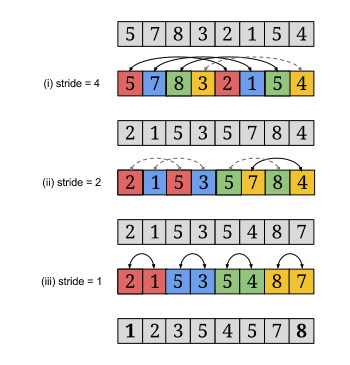
\includegraphics[width=0.5\textwidth]{images/minmax-example.png}
  \caption{Example run on an array of 8 values. 4 threads compare 2
    values at a time, swapping the values so that the smallest of them
  are to the left. At each step, the stride decreases. In the end, the
  smallest value is located at index 0, and the largest value is at
  index 7. The full arrows show values that need to be swapped, while
  the dotted shows values already in the correct place.}
  \label{minmax-example-figure}
\end{figure}


\subsection{Refinement kernels}


\subsubsection{Cross Checking}

As explained in section \ref{sect:cross-checking-theory},
cross-checking is function that compares the left and right disparity
maps, removing unreliable matches. Unreliable matches can occur from
occlusions, reflective surfaces, or a surface difficult for the used
aggregation window size to properly match.


The function is pretty straight forward:

\[ \mathlarger{| (D(x,y)_l - D(x - D(x,y)_l ,y)_r | > T} \]

At each coordinate, grab the left disparity value. The right disparity
value is then fetched at the same coordinates minus the left disparity
value. These two disparity values are compared, and if the absolute
difference is beneath some threshold (1-2 depth levels is a good
threshold), it is a good match and the left disparity value is written
to the left disparity map. If the absolute difference is greater, it's
an unreliable match and a 0 is written in that coordinate.

\begin{lstlisting}[label={lst:cross-check}, caption=Cross-checking
  function.]

  // Fist examine the left image

  int left = left_result[gid.y * WIDTH + gid.x];
  int right = right_result[gid.y * WIDTH + gid.x - left];

  if(abs(left - right) > THRESHOLD)
      new_left[gid.y * WIDTH + gid.x] = 0;
  else
      new_left[gid.y * WIDTH + gid.x] = left;


  // And the same for the right image

  left = left_result[gid.y * WIDTH + gid.x];
  right = right_result[gid.y * WIDTH + gid.x + right];

  if(abs(left - right) > THRESHOLD)
      new_right_result[gid.y * WIDTH + gid.x] = 0;
  else
      new_right_result[gid.y * WIDTH + gid.x] = right;

\end{lstlisting}

Figure \ref{fig:cross-check-results} shows the results with and
without cross-checking. The left column, especially along the left
side of depth discontinuities, contains a large spread of disparity
values. This is because the WTA strategy always selects a best match,
whether it is a correct match or not.

\begin{figure}

  \begin{subfigure}[b]{0.48\textwidth}
    \centering
    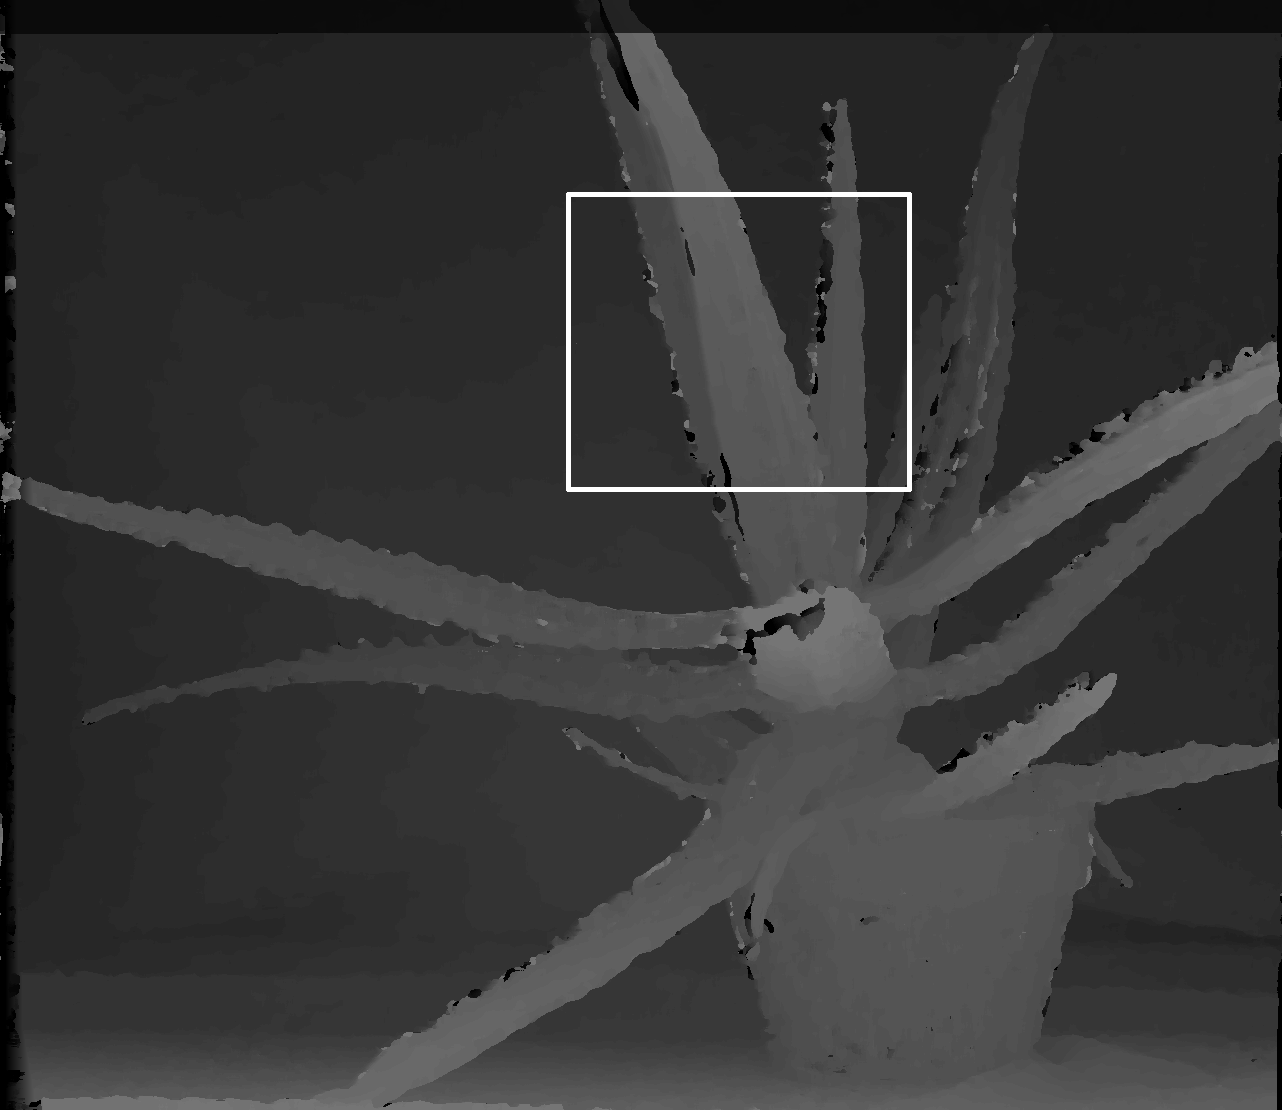
\includegraphics[width=\textwidth]{images/normal.png}
  \end{subfigure}
  ~
  \begin{subfigure}[b]{0.48\textwidth}
    \centering
    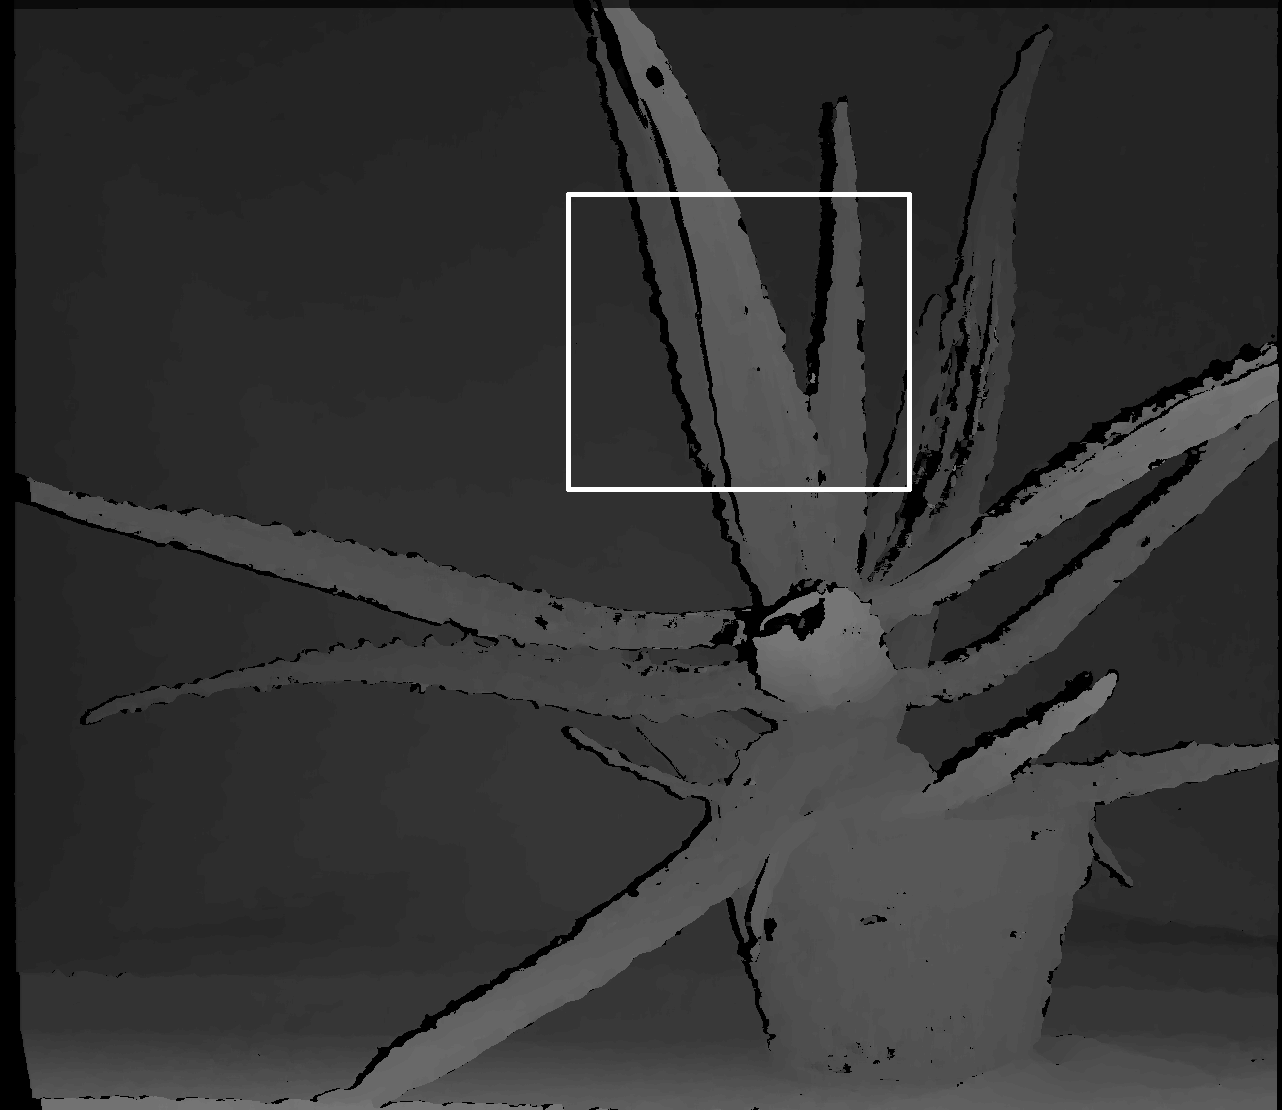
\includegraphics[width=\textwidth]{images/no-fill.png}
  \end{subfigure}

  \begin{subfigure}[b]{0.48\textwidth}
    \centering
    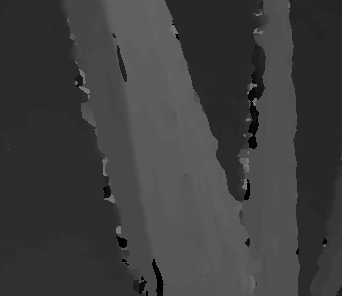
\includegraphics[width=\textwidth]{images/normal-zoomed.png}
    \caption{Without cross-checking}
  \end{subfigure}
  ~
  \begin{subfigure}[b]{0.48\textwidth}
    \centering
    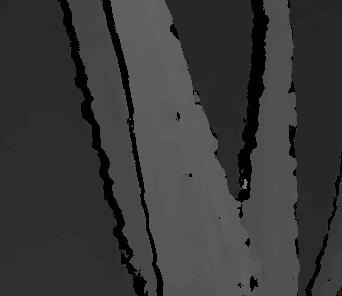
\includegraphics[width=\textwidth]{images/no-fill-zoomed.png}
    \caption{With cross-checking}
  \end{subfigure}

  \caption{Output without (column (a)) and with (column (b))
    cross-checking}

\end{figure}



\subsubsection{Occlusion Filling}

Scanline smearing. For every

\begin{figure}

  \begin{subfigure}[b]{0.48\textwidth}
    \centering
    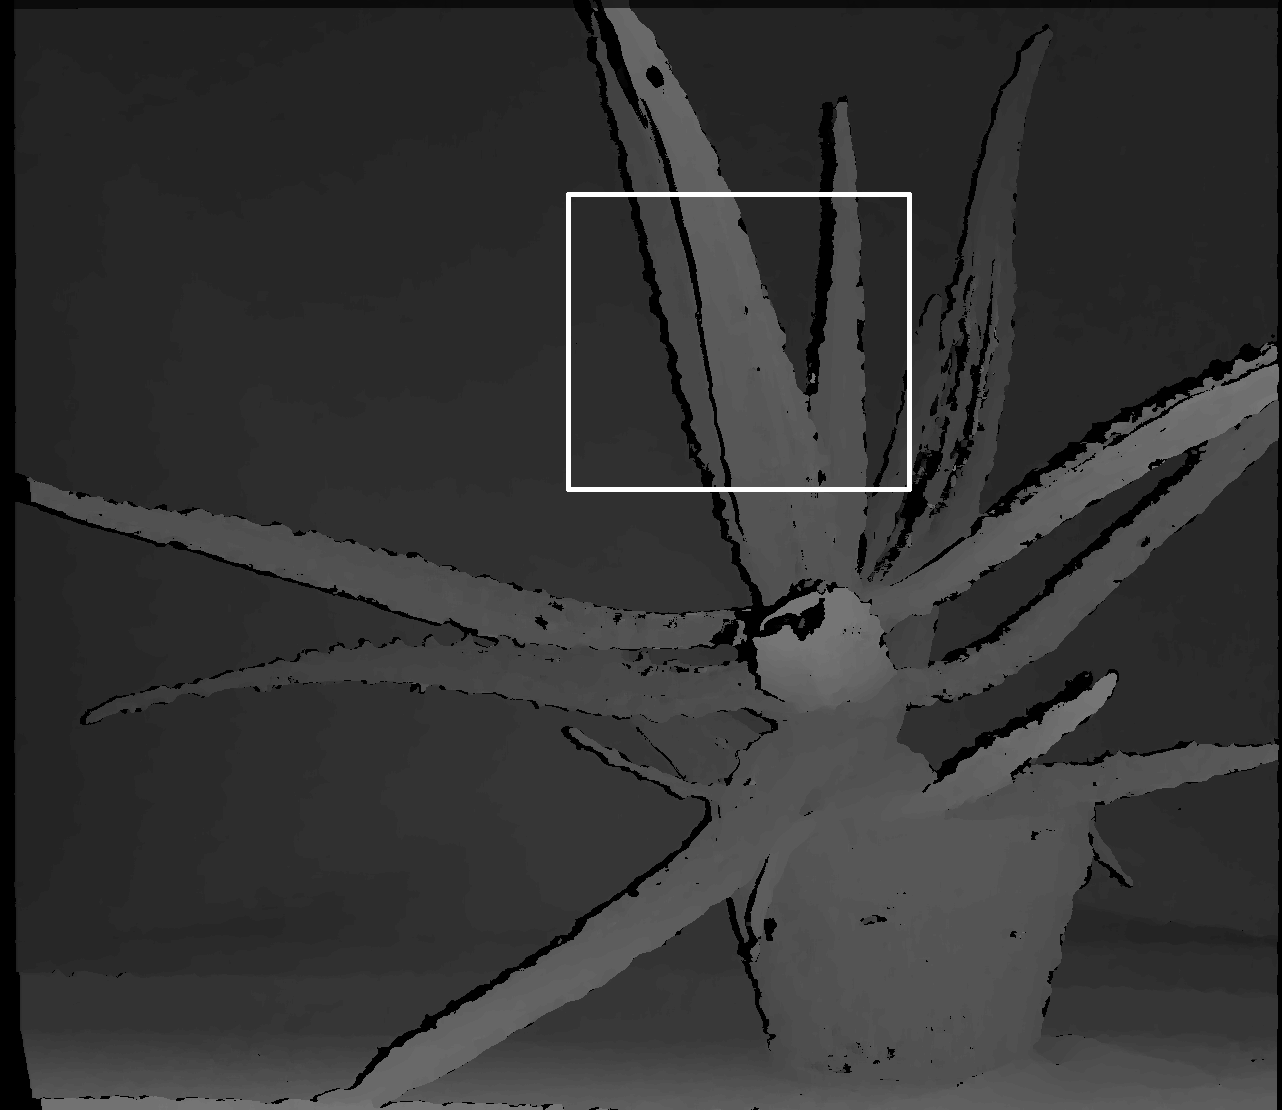
\includegraphics[width=\textwidth]{images/no-fill.png}
  \end{subfigure}
  ~
  \begin{subfigure}[b]{0.48\textwidth}
    \centering
    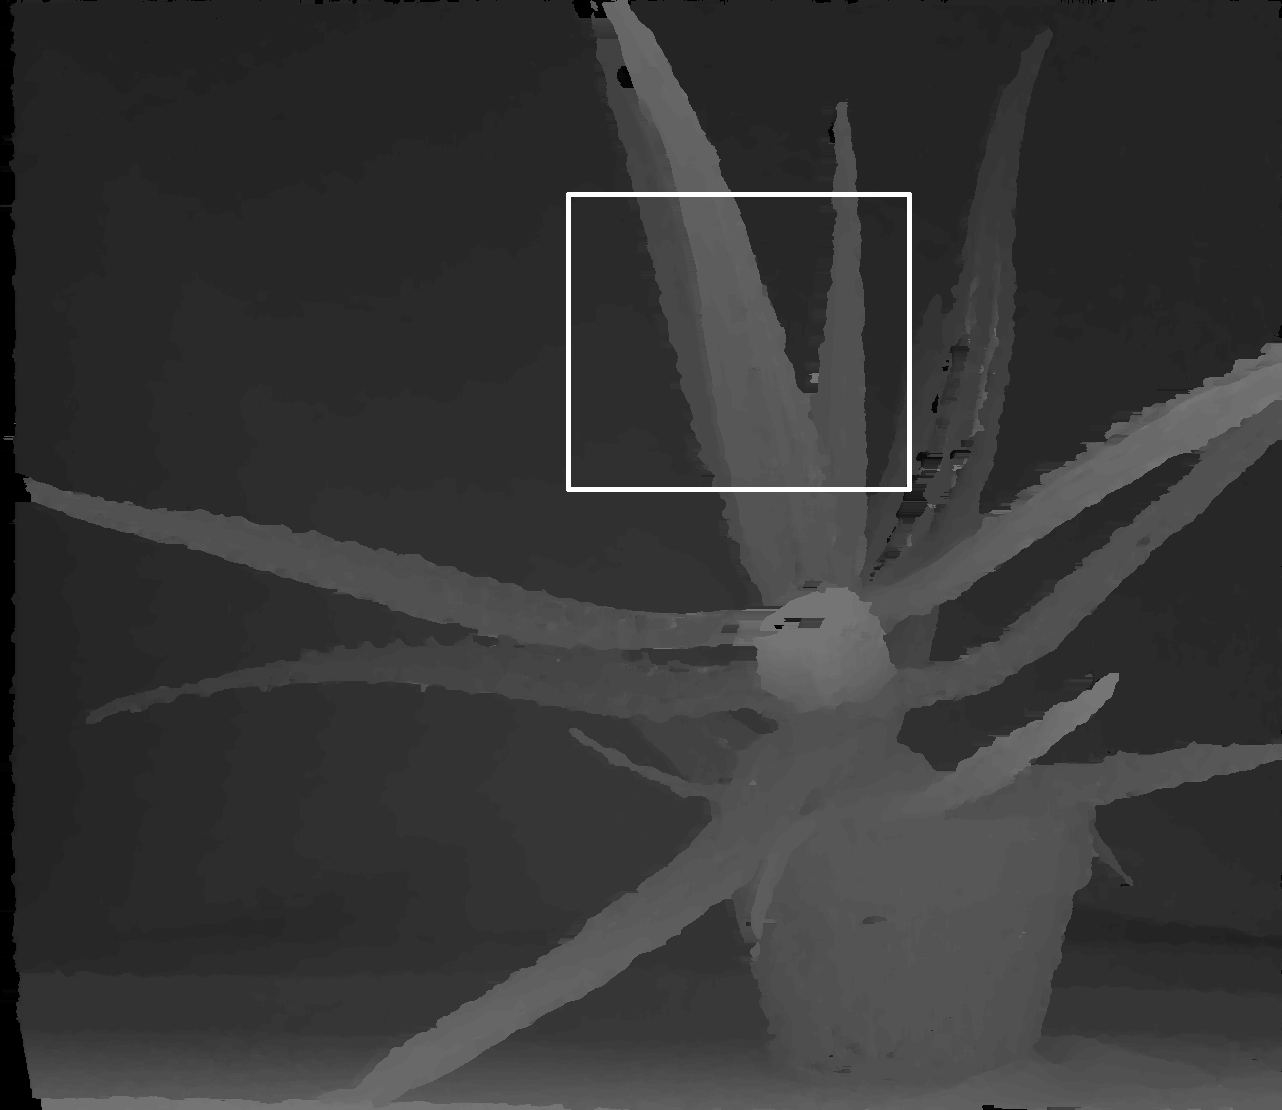
\includegraphics[width=\textwidth]{images/fill.png}
  \end{subfigure}

  \begin{subfigure}[b]{0.48\textwidth}
    \centering
    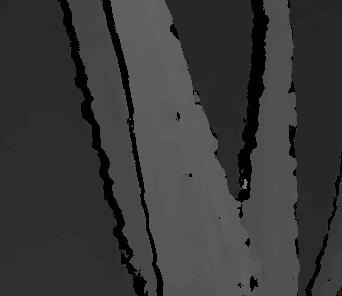
\includegraphics[width=\textwidth]{images/no-fill-zoomed.png}
    \caption{Unfilled occlusions}
  \end{subfigure}
  ~
  \begin{subfigure}[b]{0.48\textwidth}
    \centering
    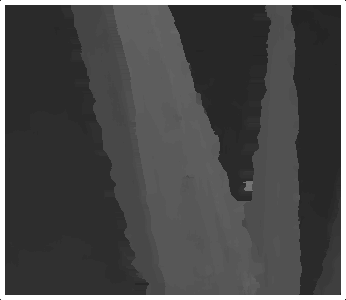
\includegraphics[width=\textwidth]{images/fill-zoomed.png}
    \caption{Filled occlusions}
  \end{subfigure}


\end{figure}



\subsubsection{Compute mask}
% Blockwise compute mask/map, workload management, creates

Sequential video frames contain a lot of redundant information,
especially when cameras remain fixed in position, always watching the
same scene.

Another way to reduce the number of computations is to avoid having to
calculate every disparity value for every frame. Sequential video
frames often have little variation. For example, the scene's
background is very likely to stay the same (unless the lighting
changes, or the camera is moved), so calculating these disparities is
a unnecessary.

One way to avoid re-calculating the same values for the next frame, is
by building a diff map. A binary image that indicates which pixels
have changed since the previous frame.
